\section{experimental details}
\label{sec:experimental_details}

\subsection*{Parameter Sweep Application and Infrastructure}
A parameter sweep application containing 50 files and 50 tasks is randomly
generated. Connections between files and tasks are random. File sizes range from
1 to 1000 megabytes and task computation requirements range from 1 to 1000 flops.

The master worker infrastructure containing 10 workers is also randomly
generated. Each worker has a compute speed ranging from 1 to 1000 flops per second
and the link between the master and each worker ranges from 1 to 1000 megabytes
per second.

When executing the GA and heuristics, the same parameter
sweep application and master worker infrastructure is used. The scheduling
logic for both the GA and the heuristics is implemented in C++
using the WRENCH API.

\subsection*{Genetic Algorithm}
Using the variation operators described in Section~\ref{sec:genetic_algorithm}, the GA itself is implemented in Python.
Additionally, Python C++ bindings
were developed to enable the GA to pass individuals into the
WRENCH simulation for fitness evaluation. Parameters for the GA used in the
experiment is described below.
\begin{table}[h]
\begin{tabular*}{\hsize}{l@{\extracolsep{\fill}}llll}
  \toprule
  \multicolumn{5}{c}{\textbf{GA Parameters}}      \\
  \midrule
  population size:    & 200 \\
  elitism:            & 0.5 \\
  parent selection:          & binary tournament \\
  mutation rate:      & 0.5 \\
  stopping condition: &150 generations \\
  \bottomrule
\end{tabular*}
\end{table}

\subsection*{Results}
After evolving over 150 generations, the GA produced an indivdidual with a
max fitness (minimum makespan) of 919.221 seconds. Max-Min resulted in an
application makespan of 493.90 seconds while Min-Min resulted in an application
makespan of 494.90 seconds. Both heuristics produced schedules that performed
about twice as good as the best individual produced by the GA, shown in
Figure~\ref{fig:results}. As the GA moved from generation to generation, it
takes a longer period of time between generations for an improvement to be
shown in the individual with the maximum fitness (shown by the slope of then blue line). It is also important to note
that when the population as a whole begins to converge onto the hightest fit
individual, there are some noticeable improvements in the hightest fit
individual in generations that immediately follow. This can be seen around generations 20, 70, and 135. An implication
of this could be such that if the GA ran for more than 150 generations, we
would likely witness the population fitness converge onto where Max-Min and Min-Min
currently stand.
\begin{figure}[t!]
  \centering
  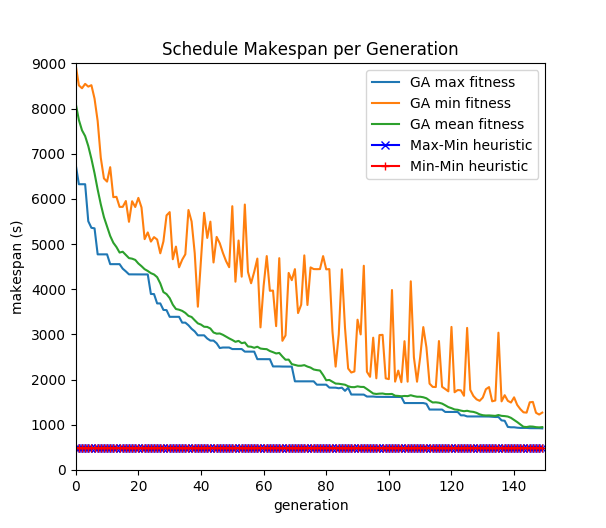
\includegraphics[width=90mm, height=80mm]{figures/results.png}
  \caption{Comparing results of the genetic algorithm against the Max-Min and Min-Min heuristics.}
  \label{fig:results}
\end{figure}
